%% 
%%  An UIT Edition example
%% 
%%  Example 04-27-26 on page 146.
%% 
%%  Copyright (C) 2012 Vo\ss 
%% 
%%  It may be distributed and/or modified under the conditions
%%  of the LaTeX Project Public License, either version 1.3
%%  of this license or (at your option) any later version.
%% 
%%  See http://www.latex-project.org/lppl.txt for details.
%% 

% Show page(s) 1,2,3

%% ==== 
\PassOptionsToClass{}{beamer}
\documentclass[serif, aspectratio=169]{beamer}
\usepackage[utf8]{inputenc}
\usepackage{textcomp}

%\StartShownPreambleCommands
\usepackage{amsmath,esint}
\usepackage[british]{babel}
\usetheme{Warsaw}
\usecolortheme{rose}

%\usetheme{metropolis}
%\usepackage{appendixnumberbeamer}

%\StopShownPreambleCommands
\usepackage{pgfplots}
\usepackage{ mathrsfs }
\usepackage{caption}
\usepackage{ragged2e}
\usepackage{gensymb}
\usepackage{color}
\usepackage{url}
\usetikzlibrary{shapes,backgrounds,calc}

\usepackage{tkz-euclide}
\usetkzobj{all}
\usepackage{tkz-fct}  
\usetikzlibrary{calc}
\usepackage{tikz,calc}

\usepackage[ruled]{algorithm2e}
\usepackage{tikz}
\usetikzlibrary{arrows.meta}
\usepackage{animate}
\DeclareMathOperator*{\minimize}{minimize}

\addtobeamertemplate{navigation symbols}{}{%
    \usebeamerfont{footline}%
    \usebeamercolor[fg]{footline}%
    \hspace{1em}%
    \insertframenumber/\inserttotalframenumber
}

\renewcommand{\thealgocf}{}

\makeatletter
\newcommand\titlegraphicii[1]{\def\inserttitlegraphicii{#1}}
\titlegraphicii{}
\setbeamertemplate{title page}
{
  \vspace{0.3in}
  \vbox{}
   %{\usebeamercolor[fg]{titlegraphic}\inserttitlegraphic\hfill\inserttitlegraphicii\par}
  \begin{centering}
    \begin{beamercolorbox}[sep=8pt,center]{title}
      \usebeamerfont{title}\inserttitle\par%
      \ifx\insertsubtitle\@empty%
      \else%
        \vskip0.25em%
        {\usebeamerfont{subtitle}\usebeamercolor[fg]{subtitle}\insertsubtitle\par}%
      \fi%     
    \end{beamercolorbox}%
    \vskip1em\par
    \begin{beamercolorbox}[sep=8pt,center]{date}
      \usebeamerfont{date}\insertdate
    \end{beamercolorbox}%\vskip0.5em
    \begin{beamercolorbox}[sep=8pt,center]{author}
      \usebeamerfont{author}\insertauthor
    \end{beamercolorbox}
    \begin{beamercolorbox}[sep=8pt,center]{institute}
      \usebeamerfont{institute}\insertinstitute
    \end{beamercolorbox}
  \end{centering}
  %\vfill
}
\makeatother
%\author{Anirban Laha and Preksha Nema \\\vspace{0.2in} Presented By: Mitesh M. Khapra}
\author{Mitesh M. Khapra}
\title{CS7015 (Deep Learning) : Lecture 3}
\subtitle{Sigmoid Neurons, Gradient Descent, Feedforward Neural Networks, Representation Power of Feedforward Neural Networks}
\institute{Department of Computer Science and Engineering\\ Indian Institute of Technology Madras}
\date{}
\titlegraphic{
\includegraphics[height=1cm,width=2cm]{images/iitm_logo.png}}
%\titlegraphicii{\includegraphics[height=1cm,width=2cm]{logo2}}


\begin{document}


\renewcommand{\thefootnote}{$\star$}

\tikzset{
	o/.style={
			shorten >=#1,
			decoration={
					markings,
					mark={
							at position 1
							with {
									\draw circle [radius=#1];
								}
						}
				},
			postaction=decorate
		},
	o/.default=2pt
}

\newcommand\derivative[5]{%
	\tkzDefPointByFct[draw](#1) \tkzGetPoint{start}
	\tkzDefPointByFct[draw](#2) \tkzGetPoint{end}
	\draw[thin,|-|,yshift=-3pt] (start) -- node[black,fill=white,#5] {#3}(start-|end);
	\draw[thin,|-|,xshift=3pt] (start-|end) -- node[black,fill=white,right] {#4}(end);
	%\draw[thin] (start) --(end); 
}

\title{Lecture 3}
\author{Mitesh M. Khapra}
\maketitle


%\begin{frame}
%Slide containing the diagrams  and then a `?'
%\end{frame}

\begin{frame}
	\begin{columns}
		\column{0.5\textwidth}
		\begin{overlayarea}{\textwidth}{\textheight}
			\textbf{Representation power of a multilayer network of perceptrons}
			\vspace{0.1in}

			\onslide<2->{\color{blue}{A multilayer network of perceptrons} \color{black}{} with a single hidden layer can be used to \color{cyan}{represent} \color{black}{} any \color{red}{boolean} \color{black}{} function \color{orange}{precisely (no errors)}} %($f(x): \{0, 1\}^n \rightarrow \{0, 1\}^m$) . \\

		\end{overlayarea}



		\column{0.5\textwidth}
		\begin{overlayarea}{\textwidth}{\textheight}
			\textbf{Representation power of a multilayer network of sigmoid neurons}
			\vspace{0.1in}

			\onslide<3->{\color{blue}{A multilayer network of neurons} \color{black}{} with a single hidden layer can be used to \color{cyan}{approximate} \color{black}{} any \color{red}{continuous} \color{black}{} function  \color{orange}{to any desired precision} \color{black}{}} %($f(x): \mathbb{R}^n \rightarrow \mathbb{R}^m$).  \\

			\vspace{0.2in}
			\onslide<4->{In other words, there is a guarantee that for any function $f(x): \mathbb{R}^n \rightarrow \mathbb{R}^m$, we can always find a neural network (with 1 hidden layer containing enough neurons) whose output g(x) satisfies $|g(x) - f(x) | < \epsilon$ !! \\}
			\vspace{0.2in}
			%(From now on in this course we will refer to a \textbf{network of neurons} as \textbf{feedforward neural networks} - though in the literature they are often referred to as \textbf{multilayer perceptrons} also) \\

			\onslide<5->{\textbf{Proof:} We will see an illustrative proof of this... [Cybenko, 1989], [Hornik, 1991]}
		\end{overlayarea}
	\end{columns}
\end{frame}


\begin{frame}
	\begin{itemize}\justifying
		\item See this link\footnote{\url{http://neuralnetworksanddeeplearning.com/chap4.html}} for an excellent illustration of this proof
		\item The discussion in the next few slides is based on the ideas presented at the above link
	\end{itemize}
\end{frame}

\begin{frame}
	\begin{columns}
		\column{0.5\textwidth}
		\begin{overlayarea}{\textwidth}{\textheight}
			\begin{onlyenv}
				\begin{figure}
					\centering
					\includegraphics<1>[scale=0.3]{./images/Plots/plot1}
					\includegraphics<2>[scale=0.3]{./images/Plots/plot1_lessbins.png}
					\includegraphics<3>[scale=0.3]{./images/Plots/plot1_morebins.png}
					\includegraphics<4->[scale=0.4]{./images/Plots/plot1_morebins_detail.png}
				\end{figure}
			\end{onlyenv}
		\end{overlayarea}

		\column{0.5\textwidth}
		\begin{overlayarea}{\textwidth}{\textheight}
			\begin{itemize}\justifying
				\item We are interested in knowing whether a network of neurons can be used to represent an arbitrary function (like the one shown in the figure)
				\item<2-> We observe that such an arbitrary function can be approximated by several ``tower'' functions
				\item<3-> More the number of such ``tower'' functions, better the approximation
				\item<4-> To be more precise, we can approximate any arbitrary function by a sum of such ``tower'' functions
			\end{itemize}
		\end{overlayarea}
	\end{columns}
\end{frame}

\begin{frame}
	\begin{columns}
		\column{0.5\textwidth}
		\begin{overlayarea}{\textwidth}{\textheight}

			\tikzstyle{neuron}=[circle,draw=red!50,fill=red!10, thick,minimum size=10mm]
			\tikzstyle{neuron1}=[circle,draw=blue!50,fill=cyan!10, thick,minimum size=10mm]
			\begin{tikzpicture}[scale=0.6]

				\onslide<3->{
					\node [neuron] (neuron1) at (10,0) {$x$};

					\draw[->] (neuron1) -- (5.7,1.6);
					\draw[->] (neuron1) -- (7.7,1.6);
					\node[text width=0.5cm] at (10,1.2) {\LARGE {.}};
					\node[text width=0.5cm] at (10.5,1.2) {\LARGE {.}};
					\node[text width=0.5cm] at (11,1.2) {\LARGE {.}};
					\draw[->] (neuron1) -- (12.7,1.6);
					\draw[->] (neuron1) -- (14.7,1.6);


					\node[text width=0.5cm] at (5.5,2.5) {Tower maker};
					\draw[gray,thick,solid] (5,1.7) rectangle (6.75,3.3);

					\node[text width=0.5cm] at (7.5,2.5) {Tower maker};
					\draw[gray,thick,solid] (7,1.7) rectangle (8.75,3.3);

					\node[text width=0.5cm] at (9.5,2.5) {\LARGE {.}};
					\node[text width=0.5cm] at (10.5,2.5) {\LARGE {.}};
					\node[text width=0.5cm] at (11.5,2.5) {\LARGE {.}};

					\node[text width=0.5cm] at (12.5,2.5) {Tower maker};
					\node[text width=0.5cm] at (12.5,2.5) {Tower maker};

					\node[text width=0.5cm] at (12.5,2.5) {Tower maker};
					\draw[gray,thick,solid] (12,1.7) rectangle (13.75,3.3);

					\node[text width=0.5cm] at (14.5,2.5) {Tower maker};
					\draw[gray,thick,solid] (14,1.7) rectangle (15.75,3.3);
				}

				\onslide<4-> {
					\node (plot) at (5.7,4.5) {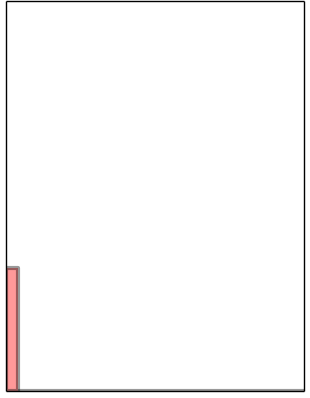
\includegraphics[scale=0.1]{p1.png}};
					\node (plot) at (7.7,4.5) {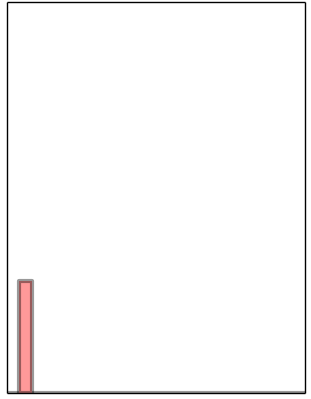
\includegraphics[scale=0.1]{p2.png}};
					\node[text width=0.5cm] at (9.5,4) {\LARGE {.}};
					\node[text width=0.5cm] at (10.5,4) {\LARGE {.}};
					\node[text width=0.5cm] at (11.5,4) {\LARGE {.}};
					\node (plot) at (12.7,4.5) {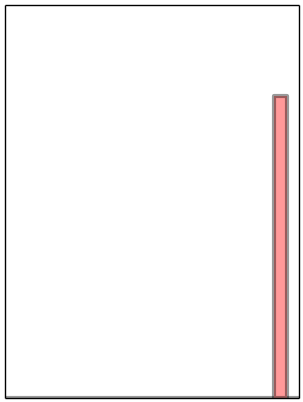
\includegraphics[scale=0.1]{p3.png}};
					\node (plot) at (14.7,4.5) {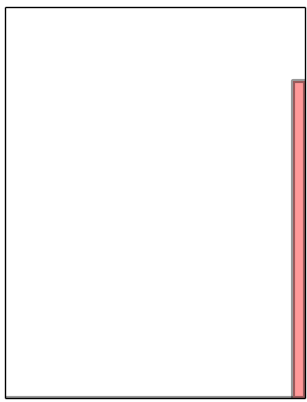
\includegraphics[scale=0.1]{p4.png}};
				}

				\onslide<6-> {
					\node [neuron1] (neuron2) at (10,7) {$+$};
					\draw[->]  (5.7,5.4) -- (neuron2);
					\draw[->]  (7.7,5.4) -- (neuron2);

					\node[text width=0.5cm] at (9.5,5.5) {\LARGE {.}};
					\node[text width=0.5cm] at (10.5,5.5) {\LARGE {.}};
					\node[text width=0.5cm] at (11.5,5.5) {\LARGE {.}};

					\draw[->]  (12.7,5.4) -- (neuron2);
					\draw[->]  (14.7,5.4) -- (neuron2);
					\draw[->]  (neuron2) -- (10,8.8) ;
				}
				\node (plot) at (10,10.5) {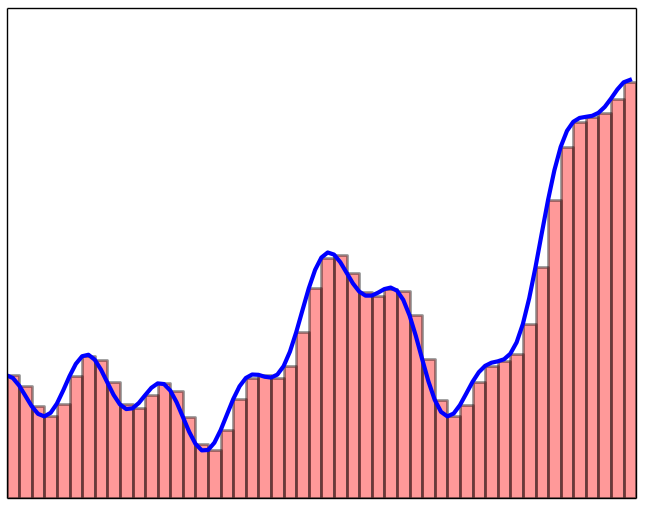
\includegraphics[width=7cm, height=2cm]{plot.png}};

			\end{tikzpicture}
		\end{overlayarea}



		\column{0.5\textwidth}
		\begin{overlayarea}{\textwidth}{\textheight}
			\begin{itemize}\justifying
				\item<1-> We make a few observations
				\item<2-> All these ``tower'' functions are similar and only differ in their heights and positions on the x-axis
				\item<3-> Suppose there is a black box which takes the original input ($x$) and constructs these tower functions
				\item<5-> We can then have a simple network which can just add them up to approximate the function
				\item<7-> Our job now is to figure out what is inside this blackbox
			\end{itemize}
		\end{overlayarea}
	\end{columns}
\end{frame}


\begin{frame}
	We will figure this out over the next few slides ...
\end{frame}

\begin{frame}
	\begin{columns}
		\column{0.5\textwidth}
		\begin{overlayarea}{\textwidth}{\textheight}
			\begin{onlyenv}
				\only<0-44>{
					\begin{figure}
						\includegraphics<1-2>[scale=0.25]{images/Plots/sig_2d/a_6}
						\foreach \n in {0,...,44} {%
								\pgfmathsetmacro\result{int(\n + 6)}
								\pgfmathsetmacro\t{int(\n + 3)}
								\includegraphics<\t>[scale=0.25]{images/Plots/sig_2d/a_\result}
							}
					\end{figure}
					\foreach \n in {0,...,44} {%
							\pgfmathsetmacro\result{int(\n + 6)}
							\pgfmathsetmacro\t{int(\n + 3)}
							\only<\t>{$w = \result, b = 0, \t$}
						}
				}
				\only<45->{
					\begin{figure}
						\foreach \n in {1,...,35} {%
								\pgfmathsetmacro\result{int(\n + 44)}
								\includegraphics<\result>[scale=0.25]{images/Plots/sig_2d/b_\n}
							}
					\end{figure}
					\foreach \n in {1,...,35} {%
							\pgfmathsetmacro\result{int(\n + 44)}
							\only<\result>{$w = 50, b = \n $}
						}
				}
			\end{onlyenv}
		\end{overlayarea}



		\column{0.5\textwidth}
		\begin{overlayarea}{\textwidth}{\textheight}
			\begin{itemize}\justifying
				\item<1-> If we take the logistic function and set $w$ to a very high value we will recover the step function
				\item<2-> Let us see what happens as we change the value of $w$
				\item<45-> Further we can adjust the value of $b$ to control the position on the x-axis at which the function transitions from 0 to 1
				      %\item Now let us see what we get by taking two such sigmoid functions (with different $b$s) and subtracting one from the other
				      %\item Voila! We have our tower function !!
				      %\item Let us see the neural network that gave us this tower function
			\end{itemize}
		\end{overlayarea}
	\end{columns}
\end{frame}


\begin{frame}
	\begin{columns}
		\column{0.5\textwidth}
		\begin{overlayarea}{\textwidth}{\textheight}

			\tikzstyle{neuron}=[circle,draw=red!50,fill=red!10, thick,minimum size=10mm]
			\tikzstyle{neuron1}=[circle,draw=blue!50,fill=cyan!10, thick,minimum size=10mm]
			\begin{tikzpicture}

				\node (plot) at (0,10) {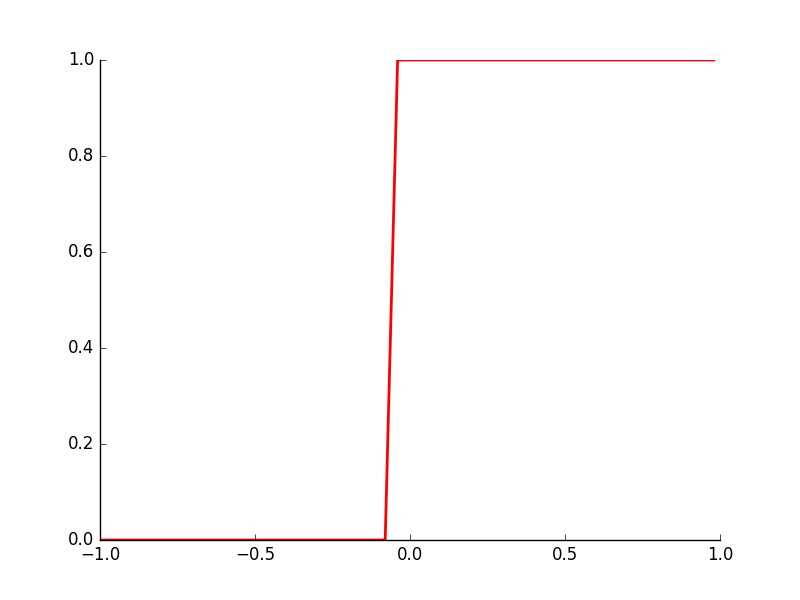
\includegraphics[width=4cm,height=4cm]{./images/Plots/1}};

				\node (plot) at (4,10) {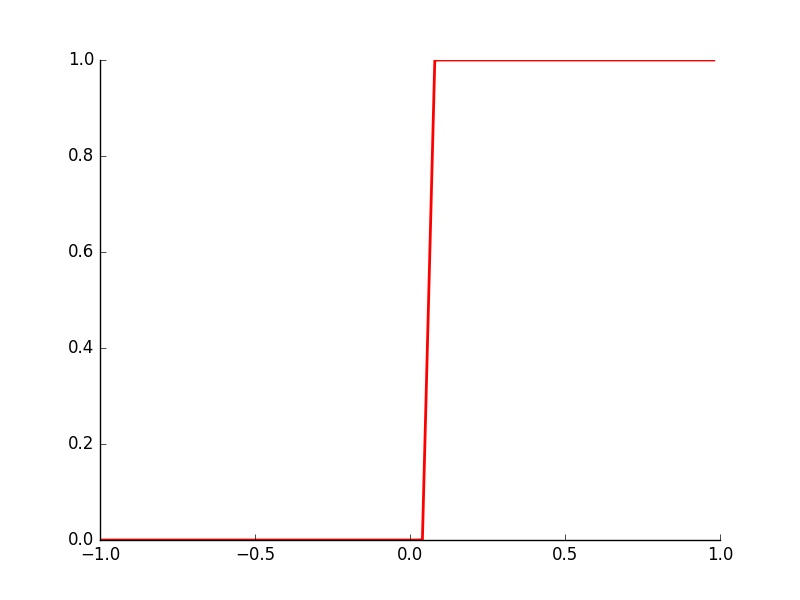
\includegraphics[width=4cm,height=4cm]{./images/Plots/2}};

				\onslide<3->{\node (plot) at (2,6) {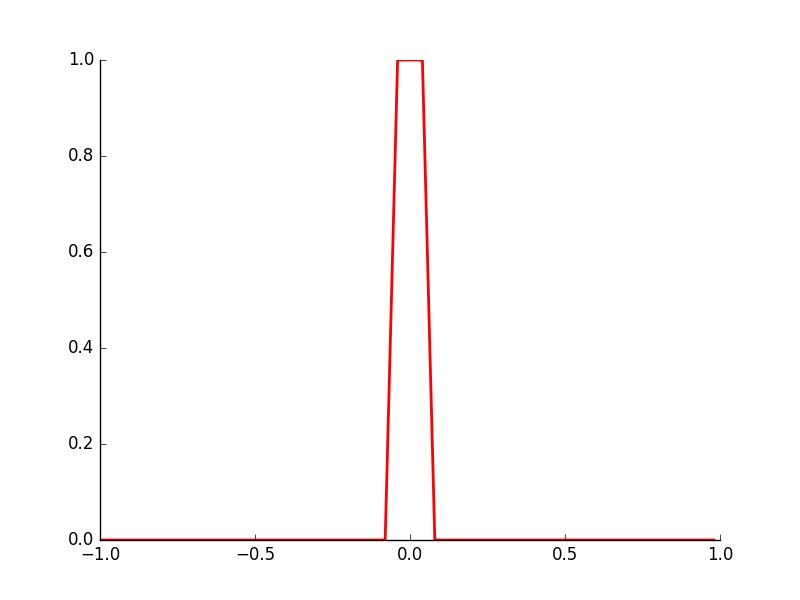
\includegraphics[width=4cm,height=4cm]{./images/Plots/tower}};}
				\onslide<2->{\draw[line width=0.2mm](2, 10) -- (2.2,10);}
				%\draw[line width=0.2mm](2.1,10.1)--(2.1,9.9);
				\onslide<3->{\draw[line width=0.2mm](2,8) -- (2.2,8);}
				\onslide<3->{\draw[line width=0.2mm](2,8.1)--(2.2,8.1);}
			\end{tikzpicture}
		\end{overlayarea}


		\column{0.5\textwidth}
		\begin{overlayarea}{\textwidth}{\textheight}
			\begin{itemize}\justifying
				\item Now let us see what we get by taking two such sigmoid functions (with different $b$s) and subtracting one from the other
				\item<4-> Voila! We have our tower function !!
			\end{itemize}
		\end{overlayarea}
	\end{columns}
\end{frame}

\begin{frame}
	\begin{itemize}\justifying
		\item Can we come up with a neural network to represent this operation of subtracting one sigmoid function from another ?
	\end{itemize}
\end{frame}


\begin{frame}
	\begin{figure}
		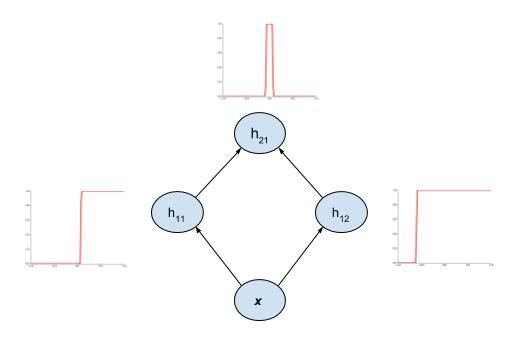
\includegraphics[scale=0.5]{images/Plots/nn2d}
	\end{figure}
\end{frame}

%\begin{frame}
%Later on in the assignment you will show that you could have done with just one hidden layer instead of two! 
%\end{frame}

\begin{frame}
	What if we have more than 1 input ?
\end{frame}


\begin{frame}
	\begin{columns}
		\column{0.5\textwidth}
		\begin{overlayarea}{\textwidth}{\textheight}
			\begin{onlyenv}
				\only<0-26>{
					\begin{figure}
						\includegraphics<1-3>[scale=0.25]{images/Plots/one/2}
						\foreach \n in {4,...,25} {%
								\pgfmathsetmacro\result{int(\n - 1)}
								\includegraphics<\n>[scale=0.25]{images/Plots/one/\result}
							}
						\includegraphics<26>[scale=0.25]{images/Plots/one/25}
					\end{figure}
					\foreach \n in {3,...,25} {%
							\pgfmathsetmacro\result{int(\n - 1)}
							\only<\n>{$w_1 = \result, w_2 = 0, b = 0 $}
						}
				}
				\only<27->{
					\begin{figure}
						\foreach \n in {0,...,9} {%
								\pgfmathsetmacro\result{int(\n + 27)}
								\includegraphics<\result>[scale=0.25]{images/Plots/two/\n}
							}
					\end{figure}
					\foreach \n in {0,...,9} {%
							\pgfmathsetmacro\result{int(\n + 27)}
							\pgfmathsetmacro\b{int(\n * 5)}
							\only<\result>{$w_1 = 25, w_2 = 0, b = \b $}
						}
				}
			\end{onlyenv}
		\end{overlayarea}



		\column{0.5\textwidth}
		\begin{overlayarea}{\textwidth}{\textheight}
			\begin{itemize}\justifying
				\item<1-> This is what a 3-dimensional sigmoid looks like
				\item<2-> We need to figure out how to get a 3-dimensional tower
				\item<3-> First, let us set $w_2$ to 0 and see if we can get a two dimensional step function
				\item<26-> What would happen if we change $b$ ?
				      %\item Now let us see what we get by taking two such sigmoid functions (with different $b$s) and subtracting one from the other
				      %\item Voila! We have our tower function !!
				      %\item Let us see the neural network that gave us this tower function
			\end{itemize}
		\end{overlayarea}
	\end{columns}
\end{frame}

\begin{frame}
	\begin{columns}
		\column{0.5\textwidth}
		\begin{overlayarea}{\textwidth}{\textheight}

			\tikzstyle{neuron}=[circle,draw=red!50,fill=red!10, thick,minimum size=10mm]
			\tikzstyle{neuron1}=[circle,draw=blue!50,fill=cyan!10, thick,minimum size=10mm]
			\begin{tikzpicture}

				\node (plot) at (0,10) {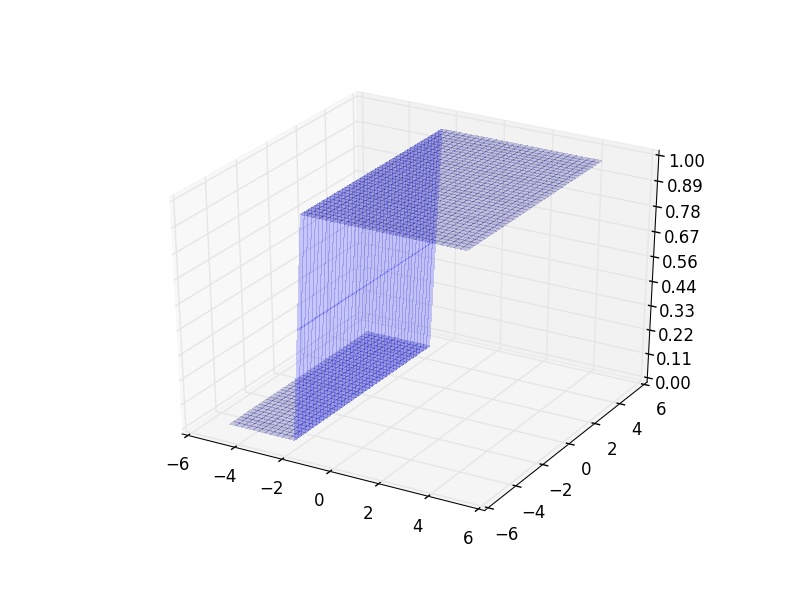
\includegraphics[width=4cm,height=4cm]{./images/Plots/three/x1}};

				\node (plot) at (4,10) {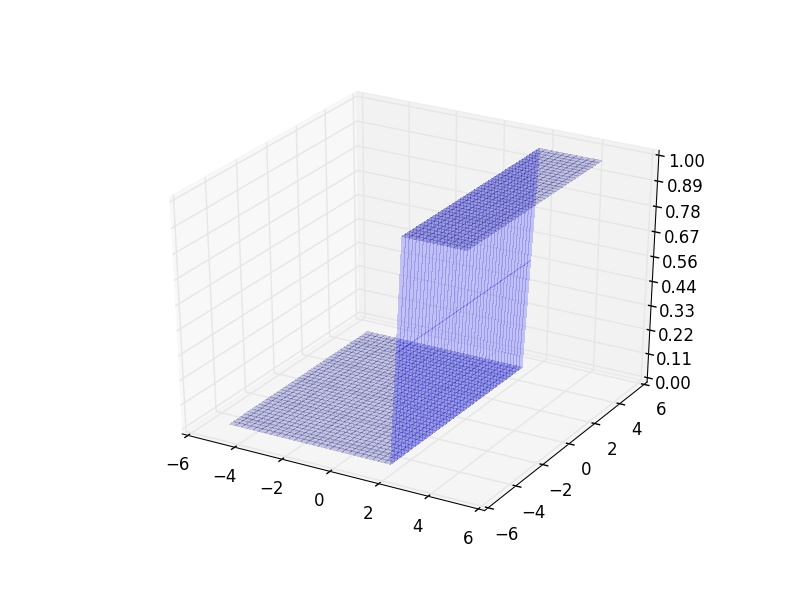
\includegraphics[width=4cm,height=4cm]{./images/Plots/three/x2}};

				\onslide<3->{\node (plot) at (2,6) {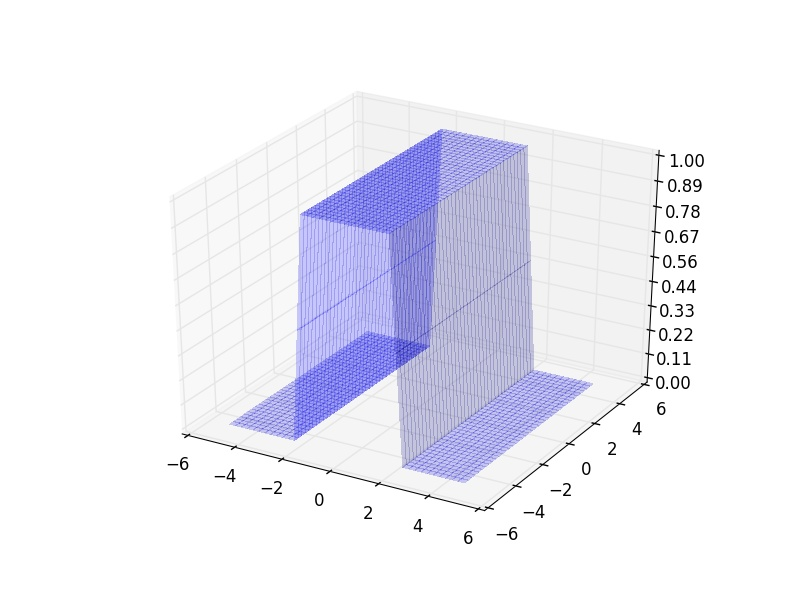
\includegraphics[width=4cm,height=4cm]{./images/Plots/three/xjoin}};}
				\onslide<2->{\draw[line width=0.2mm](2, 10) -- (2.2,10);}
				%\draw[line width=0.2mm](2.1,10.1)--(2.1,9.9);
				\onslide<3->{\draw[line width=0.2mm](2,8) -- (2.2,8);}
				\onslide<3->{\draw[line width=0.2mm](2,8.1)--(2.2,8.1);}
			\end{tikzpicture}
		\end{overlayarea}


		\column{0.5\textwidth}
		\begin{overlayarea}{\textwidth}{\textheight}
			\begin{itemize}\justifying
				\item<1-> What if we take two such step functions (with different $b$ values) and subtract one from the other
				\item<4-> We still don't get a tower (or we get a tower which is open from two sides)
				      %\item Now let us see what we get by taking two such sigmoid functions (with different $b$s) and subtracting one from the other
				      %\item Voila! We have our tower function !!
				      %\item Let us see the neural network that gave us this tower function
			\end{itemize}
		\end{overlayarea}
	\end{columns}
\end{frame}


\begin{frame}
	\begin{columns}
		\column{0.5\textwidth}
		\begin{overlayarea}{\textwidth}{\textheight}
			\begin{onlyenv}
				\only<0-26>{
					\begin{figure}
						\includegraphics<1-3>[scale=0.25]{images/Plots/five/2}
						\foreach \n in {4,...,25} {%
								\pgfmathsetmacro\result{int(\n - 1)}
								\includegraphics<\n>[scale=0.25]{images/Plots/five/\result}
							}
						\includegraphics<26>[scale=0.25]{images/Plots/five/25}
					\end{figure}
					\foreach \n in {3,...,25} {%
							\pgfmathsetmacro\result{int(\n - 1)}
							\only<\n>{$w_1 = 0, w_2 = \result, b = 0 $}
						}
				}
				\only<27->{
					\begin{figure}
						\foreach \n in {0,...,9} {%
								\pgfmathsetmacro\result{int(\n + 27)}
								\includegraphics<\result>[scale=0.25]{images/Plots/six/\n}
							}
					\end{figure}
					\foreach \n in {0,...,9} {%
							\pgfmathsetmacro\result{int(\n + 27)}
							\pgfmathsetmacro\b{int(\n * 5)}
							\only<\result>{$w_1 = 0, w_2 = 25, b = \b $}
						}
				}
			\end{onlyenv}
		\end{overlayarea}



		\column{0.5\textwidth}
		\begin{overlayarea}{\textwidth}{\textheight}
			\begin{itemize}\justifying
				\item<1-> Now let us set $w_1$ to 0 and adjust $w_2$ to get a 3-dimensional step function with a different orientation
				\item<26-> And now we change $b$
			\end{itemize}
		\end{overlayarea}
	\end{columns}
\end{frame}


\begin{frame}
	\begin{columns}
		\column{0.5\textwidth}
		\begin{overlayarea}{\textwidth}{\textheight}

			\tikzstyle{neuron}=[circle,draw=red!50,fill=red!10, thick,minimum size=10mm]
			\tikzstyle{neuron1}=[circle,draw=blue!50,fill=cyan!10, thick,minimum size=10mm]
			\begin{tikzpicture}

				\node (plot) at (0,10) {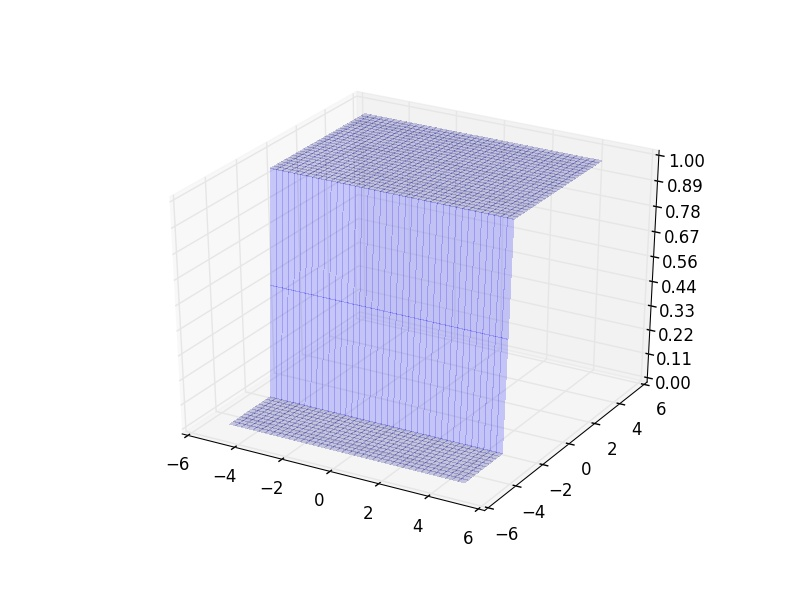
\includegraphics[width=4cm,height=4cm]{./images/Plots/three/y1}};

				\node (plot) at (4,10) {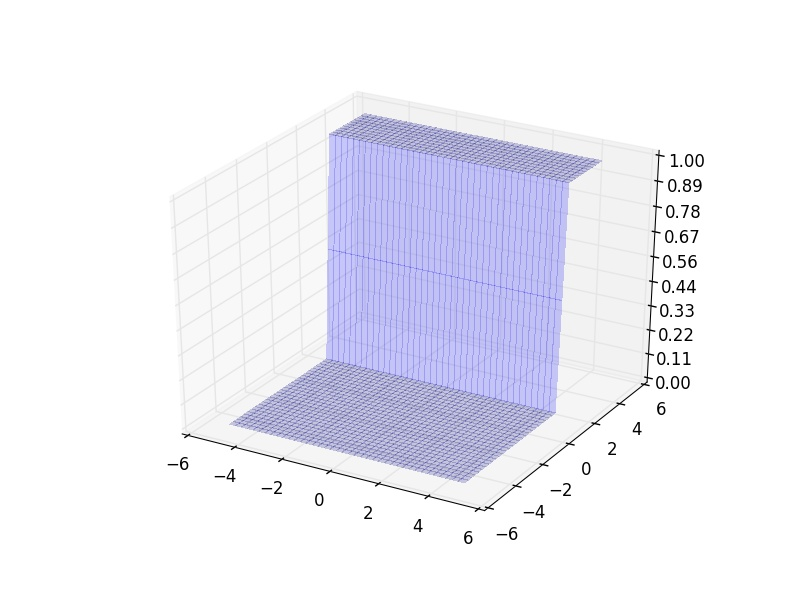
\includegraphics[width=4cm,height=4cm]{./images/Plots/three/y2}};

				\onslide<3->{\node (plot) at (2,6) {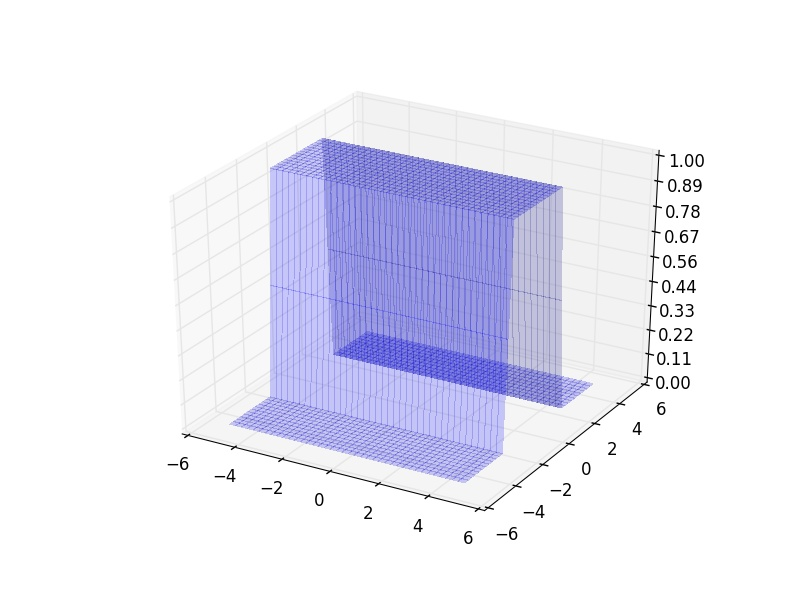
\includegraphics[width=4cm,height=4cm]{./images/Plots/three/yjoin}};}
				\onslide<2->{\draw[line width=0.2mm](2, 10) -- (2.2,10);}
				%\draw[line width=0.2mm](2.1,10.1)--(2.1,9.9);
				\onslide<3->{\draw[line width=0.2mm](2,8) -- (2.2,8);}
				\onslide<3->{\draw[line width=0.2mm](2,8.1)--(2.2,8.1);}
			\end{tikzpicture}
		\end{overlayarea}


		\column{0.5\textwidth}
		\begin{overlayarea}{\textwidth}{\textheight}
			\begin{itemize}\justifying
				\item<1-> Again, what if we take two such step functions (with different $b$ values) and subtract one from the other
				\item<4-> We still don't get a tower (or we get a tower which is open from two sides)
				\item<5-> Notice that this open tower has a different orientation from the previous one
				      %\item Now let us see what we get by taking two such sigmoid functions (with different $b$s) and subtracting one from the other
				      %\item Voila! We have our tower function !!
				      %\item Let us see the neural network that gave us this tower function
			\end{itemize}
		\end{overlayarea}
	\end{columns}
\end{frame}


\begin{frame}
	\begin{columns}
		\column{0.5\textwidth}
		\begin{overlayarea}{\textwidth}{\textheight}

			\only<1-5>{
			\tikzstyle{neuron}=[circle,draw=red!50,fill=red!10, thick,minimum size=10mm]
			\tikzstyle{neuron1}=[circle,draw=blue!50,fill=cyan!10, thick,minimum size=10mm]
			\begin{tikzpicture}

				\node (plot) at (0,10) {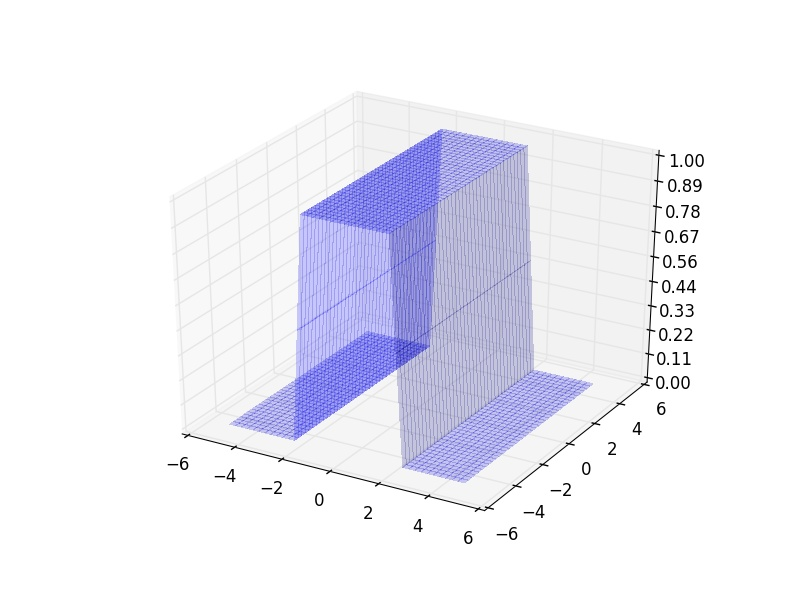
\includegraphics[width=4cm,height=4cm]{./images/Plots/three/xjoin}};

				\node (plot) at (4,10) {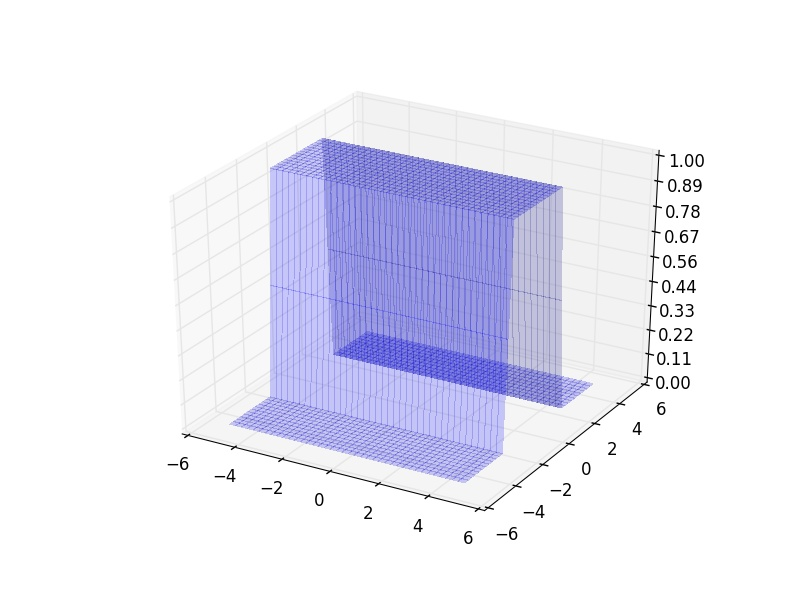
\includegraphics[width=4cm,height=4cm]{./images/Plots/three/yjoin}};

				\onslide<3->{\node (plot) at (2,6) {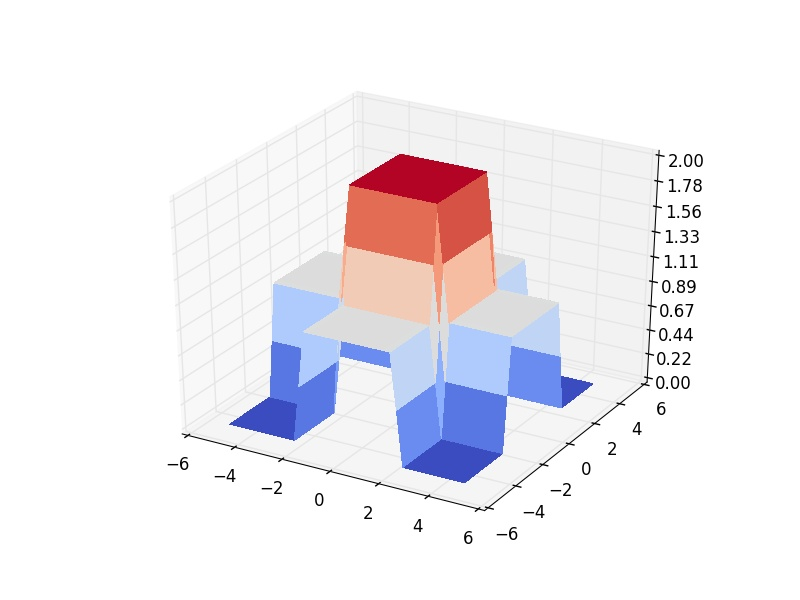
\includegraphics[width=4cm,height=4cm]{./images/Plots/three/xpyjoin}};}
				\onslide<2->{\draw[line width=0.2mm](2, 10) -- (2.2,10);}
				%\draw[line width=0.2mm](2.1,10.1)--(2.1,9.9);
				\onslide<3->{\draw[line width=0.2mm](2,8) -- (2.2,8);}
				\onslide<3->{\draw[line width=0.2mm](2,8.1)--(2.2,8.1);}
			\end{tikzpicture}
			}
			\only<6->{
				\begin{figure}
					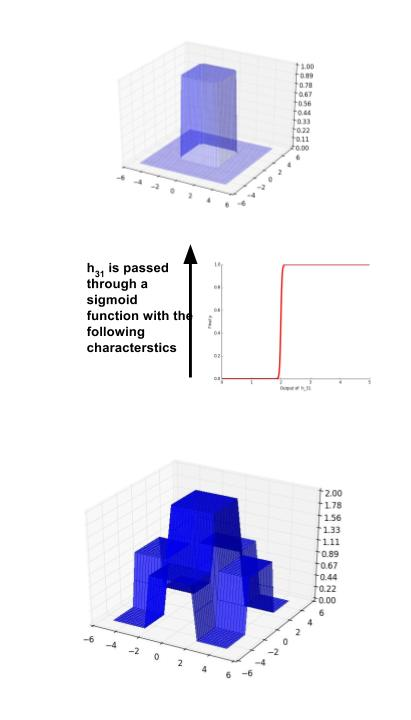
\includegraphics[scale=0.3]{./images/Plots/four/t_add}
				\end{figure}

			}
		\end{overlayarea}


		\column{0.5\textwidth}
		\begin{overlayarea}{\textwidth}{\textheight}
			\begin{itemize}\justifying
				\item<1-> Now what will we get by adding two such open towers ?
				\item<4-> We get a tower standing on an elevated base
				\item<5-> We can now pass this output through another sigmoid neuron to get the desired tower !
				\item<7-> We can now approximate any function by summing up many such towers
				      %\item Now let us see what we get by taking two such sigmoid functions (with different $b$s) and subtracting one from the other
				      %\item Voila! We have our tower function !!
				      %\item Let us see the neural network that gave us this tower function
			\end{itemize}
		\end{overlayarea}
	\end{columns}
\end{frame}

\begin{frame}
	\begin{columns}
		\column{0.5\textwidth}
		\begin{overlayarea}{\textwidth}{\textheight}
			\begin{figure}
				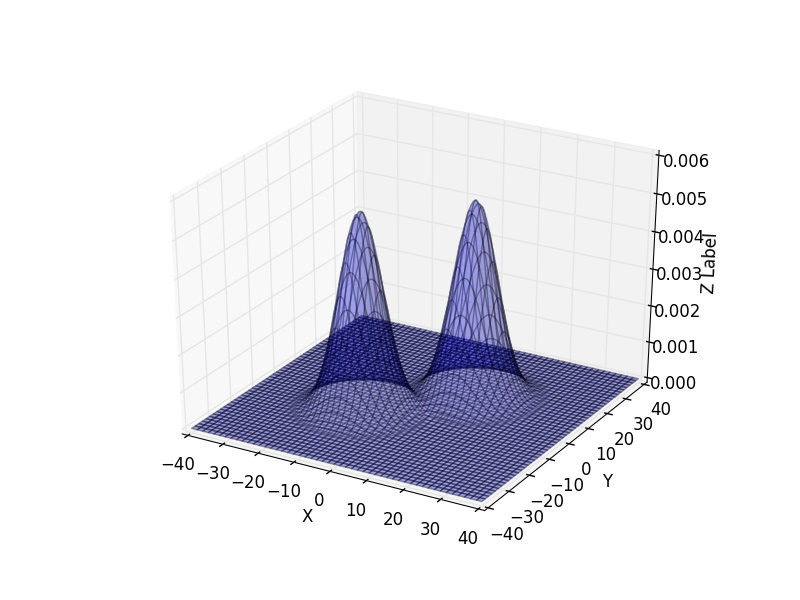
\includegraphics[scale=0.25]{images/Plots/2bells}
			\end{figure}

		\end{overlayarea}

		\column{0.5\textwidth}
		\begin{overlayarea}{\textwidth}{\textheight}
			\begin{itemize}\justifying
				\item For example, we could approximate the following function using a sum of several towers
			\end{itemize}
		\end{overlayarea}
	\end{columns}
\end{frame}

\begin{frame}
	\begin{itemize}\justifying
		\item Can we come up with a neural network to represent this entire procedure of constructing a 3 dimensional tower ?
	\end{itemize}
\end{frame}

\begin{frame}
	\begin{figure}
		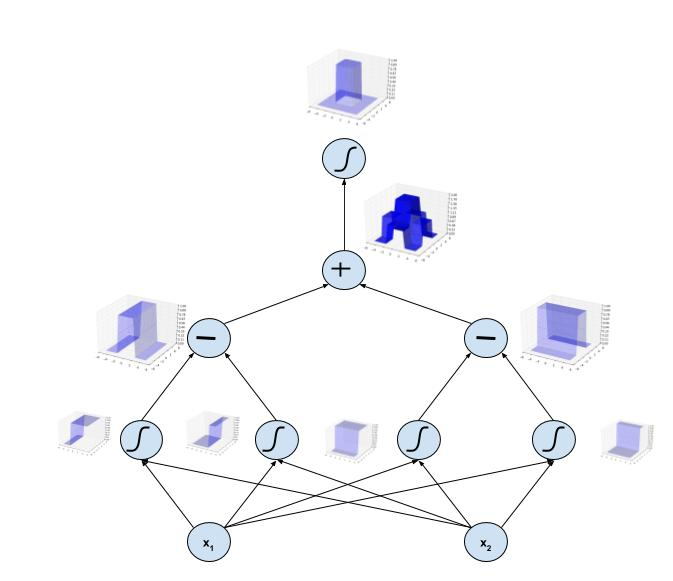
\includegraphics[scale=0.25]{images/Plots/nn_step}
	\end{figure}
\end{frame}

\begin{frame}
	\begin{figure}
		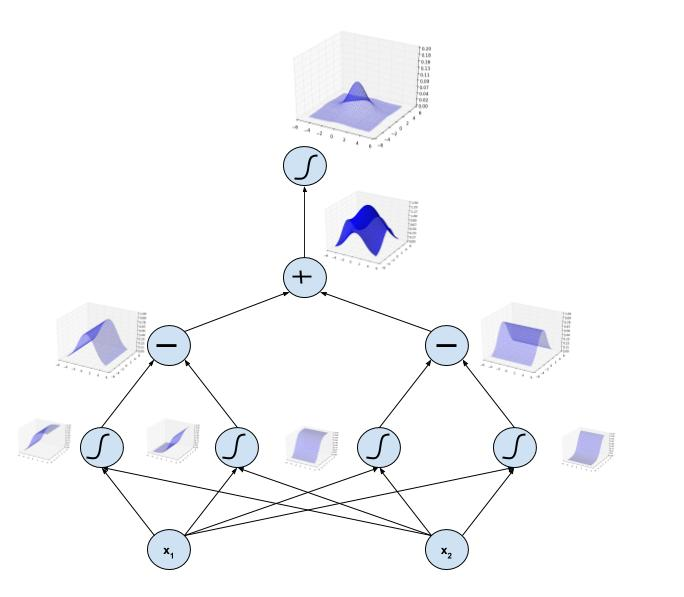
\includegraphics[scale=0.25]{images/Plots/nn_g}
	\end{figure}
\end{frame}


\begin{frame}
	\begin{block}{Think}
		\begin{itemize}\justifying
			\item For 1 dimensional input we needed 2 neurons to construct a tower
			\item For 2 dimensional input we needed 4 neurons to construct a tower
			\item How many neurons will you need to construct a tower in $n$ dimensions ?
		\end{itemize}
	\end{block}
\end{frame}

\begin{frame}
	\begin{block}{Time to retrospect}
		\begin{itemize}\justifying
			\item Why do we care about approximating any arbitrary function ?
			\item Can we tie all this back to the classification problem that we have been dealing with ?
		\end{itemize}
	\end{block}
\end{frame}


\begin{frame}
	\begin{columns}
		\column{0.5\textwidth}
		\begin{overlayarea}{\textwidth}{\textheight}

			\begin{figure}
				\includegraphics<1-2>[scale=0.10]{images/Plots/scatter}
				\includegraphics<3->[scale=0.10]{images/Plots/sig1.png}
			\end{figure}
			\vspace{-0.2in}
			\begin{itemize}\justifying
				\item We are interested in separating the blue points from the red points
				\item<2-> Suppose we use a single sigmoidal neuron to approximate the relation between $x = [x_1, x_2]$ and $y$
				\item<4-> Obviously, there will be errors (some blue points get classified as 1 and some red points get classified as 0)
				      %This will what a single neuron will give us $y = \frac{1}{1 + e^{-(w_2*x_2 + w_1*x_1 + w_0)}}$
			\end{itemize}

		\end{overlayarea}



		\column{0.5\textwidth}
		\begin{overlayarea}{\textwidth}{\textheight}
			\begin{figure}
				\includegraphics<5->[scale=0.10]{images/Plots/g2.png}
			\end{figure}
			\vspace{-0.2in}

			\begin{itemize}\justifying
				\item<5-> This is what we actually want
				\item<6-> The illustrative proof that we just saw tells us that we can have a neural network with two hidden layers which can approximate the above function by a sum of towers
				\item<7-> Which means we can have a neural network which can exactly separate the blue points from the red points !!
			\end{itemize}
		\end{overlayarea}
	\end{columns}
\end{frame}


\if 0
	\begin{frame}
		\begin{columns}
			\column{0.5\textwidth}
			\begin{overlayarea}{\textwidth}{\textheight}
			\end{overlayarea}



			\column{0.5\textwidth}
			\begin{overlayarea}{\textwidth}{\textheight}
				\begin{itemize}\justifying
					\item 1
				\end{itemize}
			\end{overlayarea}
		\end{columns}
	\end{frame}
	perceptron function and sigmoid function (continuous differentiable)
	terminology b instead of w0
	something about different loss functions
	something about non-linearities
	bigger scheme of things
	representation power
	the hat diagrams
	add assignment for two layered network

	Column1: This is what a single neural network can do
	Column2: This is what we want

	What is the data is even more difficult (show several bumps)

	The function y can be seen as an addition of several such small bump functions (show it visually)



	Proposition: if we can have a network which can approximate sa bump then we can combine several such networks together to

	Question: Can we have a network of neurons which can represent such arbitrary functions
	Side by side definitions of boolean and real UAT
	Caveats: it does not tell us anything about the number of neurons in the layer


	#Study MAterial
	Sigmoid function
	Code for plotting sigmoid function
	Can be interpreted as a probablity
\fi

\end{document}


